
%%%%%%% Standard Packages
\usepackage{amsmath}       % I think this gives me some symbols
\usepackage{amsthm}        % Does theorem stuff
\usepackage{amssymb}       % more symbols and fonts
\usepackage{amsfonts}
\usepackage[all]{xy}
\usepackage{xspace}
\usepackage{calc}
\usepackage{comment}
\usepackage{pgfplots}
\usepgflibrary{fpu}

\usepackage{ifthen}		% For if-then-else statements in making commands. 

\setlength{\topskip}{0pt}
\setlength{\footskip}{30pt}
\headheight=0pt
\topmargin=0pt
\headsep=18pt
\textheight=603pt %% 792pt to page, 648 is 9in
\textwidth=420pt  %% 612pt to page, 468pt is 6.5in
\oddsidemargin=25pt
\evensidemargin=25pt

\pagestyle{plain}

% Useful for commenting out large chunks of code
\newcommand\ignore[1]{}

  
\DeclareRobustCommand{\SkipTocEntry}[5]{}

	
	
%%%%%% Tikz !!! Commands and Macros %%%%%%%%%%%%%
\usepackage{tikz}
\usetikzlibrary{matrix}
\usetikzlibrary{arrows,backgrounds,patterns,scopes,external,
    decorations.pathreplacing,
    decorations.pathmorphing
}
\tikzexternalize[prefix=Pictures/]

\newlength{\fuzzwidth}
\setlength{\fuzzwidth}{2.5pt}
\newlength{\arrowlength}
\setlength{\arrowlength}{8pt}
\newlength{\arrowwidth}
\setlength{\arrowwidth}{.75pt}
\newlength{\pointrad}
\setlength{\pointrad}{1.5pt}
\newlength{\linewid}
\setlength{\linewid}{1.5pt}
\newlength{\circlerad}
\setlength{\circlerad}{16pt}
\newlength{\smcirclerad}
\setlength{\smcirclerad}{8pt}
\newcommand{\fillcolor}{black!60}
\newcommand{\fuzzcolor}{black!25}
\newcommand{\arrowcolor}{black!25}
\newcommand{\covercolor}{black!0}
\newcommand{\graycolor}{black!55}
\newcommand{\graylightcolor}{black!40}


\newcommand{\coverwidthfuzz}{6pt}
\newcommand{\coverwidth}{3.5pt}
\newcommand{\coverwidththin}{3.25pt}
\newcommand{\coverwidththick}{3.75pt}

\newlength{\linewidthin}
\setlength{\linewidthin}{1.25pt}
\newlength{\linewidthick}
\setlength{\linewidthick}{1.75pt}



\tikzset{
	coverline/.style={
	preaction={draw,line width=\coverwidth,\covercolor}}, 
	coverlinethin/.style={
	preaction={draw,line width=\coverwidththin,\covercolor}}, 
	coverlinethick/.style={
	preaction={draw,line width=\coverwidththick,\covercolor}}, 
	coverlineleft/.style={
	preaction={draw,line width=\coverwidthfuzz,\covercolor,decorate,decoration={curveto,amplitude=0,raise=.35*\fuzzwidth}}}, %%% Notice this number was tweaked, 	
coverlinelefttail/.style={
	preaction={draw,line width=\coverwidthfuzz,\covercolor,decorate,decoration={curveto,amplitude=0,raise=.35*\fuzzwidth,pre=moveto,pre length=2pt}}}, %%% Notice this number was tweaked, probably will not look good if parameters change.  Again here, pre removes the raise option.
        fuzzlefttail/.style={
        preaction={draw,line width=\fuzzwidth,\fuzzcolor,decorate,decoration={curveto,pre=moveto,pre length=2pt,amplitude=0,raise=.5*\fuzzwidth}}}, %%% This does not work --- somehow pre breaks the raise function.
        linestylethin/.style={line width=\linewidthin},
        linestylethick/.style={line width=\linewidthick},
        linestylegray/.style={line width=\linewid,\graycolor},
        linestylegraylight/.style={line width=\linewid,\graylightcolor}
}
\tikzset{
        fuzzright/.style={
        preaction={draw,line width=\fuzzwidth,\fuzzcolor,decorate,decoration={curveto,amplitude=0,raise=-.5*\fuzzwidth}}},
        fuzzleft/.style={
        preaction={draw,line width=\fuzzwidth,\fuzzcolor,decorate,decoration={curveto,amplitude=0,raise=.5*\fuzzwidth}}},
        fuzzrightpre/.style={ %%% Doesn't work
        preaction={draw,line width=2pt,\fuzzcolor,decorate,decoration={curveto,amplitude=0,raise=-1pt,pre=moveto,pre length=12pt}}},
        fuzzleftpre/.style={ %%% Doesn't work
        preaction={draw,line width=2pt,\fuzzcolor,decorate,decoration={curveto,post=moveto,post length=32pt,amplitude=0,raise=1pt}}},        
        outstyle/.style={\arrowcolor, line width=\arrowwidth},
        linestyle/.style={line width=\linewid}
}

\newcommand{\lilarrow}{
\draw[->] (0,0) -- (1,0);
}

\newcommand{\cb}{\raisebox{.6ex-.5\height}}


\newcommand{\arxiv}[1]{\href{http://arxiv.org/abs/#1}{\tt arXiv:\nolinkurl{#1}}}
\newcommand{\doi}[1]{\href{http://dx.doi.org/#1}{{\tt DOI:#1}}}
\newcommand{\euclid}[1]{\href{http://projecteuclid.org/getRecord?id=#1}{{\tt #1}}}
\newcommand{\mathscinet}[1]{\href{http://www.ams.org/mathscinet-getitem?mr=#1}{\tt #1}}
\newcommand{\googlebooks}[1]{(preview at \href{http://books.google.com/books?id=#1}{google books})}



%%%% These draw triple or quadruple set of arrows of length 0.5 cm
\DeclareMathOperator{\rightdoublearrows} {{\; 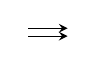
\begin{tikzpicture} \foreach \y in {0.05, 0.15} { \draw [-stealth] (0, \y) -- +(0.5, 0);} \; \end{tikzpicture}}}
\DeclareMathOperator{\leftdoublearrows} {{\; 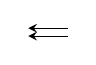
\begin{tikzpicture} \foreach \y in {0.05, 0.15} { \draw [stealth-] (0, \y) -- +(0.5, 0);} \; \end{tikzpicture}}}
\DeclareMathOperator{\righttriplearrows} {{\; 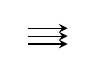
\begin{tikzpicture} \foreach \y in {0, 0.1, 0.2} { \draw [-stealth] (0, \y) -- +(0.5, 0);} \; \end{tikzpicture}}}
\DeclareMathOperator{\lefttriplearrows} {{\; 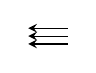
\begin{tikzpicture} \foreach \y in {0, 0.1, 0.2} { \draw [stealth-] (0, \y) -- +(0.5, 0);} \; \end{tikzpicture}}}
\DeclareMathOperator{\rightquadarrows} {{\; 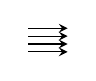
\begin{tikzpicture} \foreach \y in {-0.05, 0.05, 0.15, 0.25} { \draw [-stealth] (0, \y) -- +(0.5, 0);} \; \end{tikzpicture}}}
\DeclareMathOperator{\leftquadarrows} {{\; 
\begin{tikzpicture} \foreach \y in {-0.05, 0.05, 0.15, 0.25} { \draw [stealth-] (0, \y) -- +(0.5, 0);} \; \end{tikzpicture}}}

%%%%%%% End TikZ Commands and Macros %%%%%%%%%%%%%



%%%%%%%%%%%%%%%%%%%%%% Theorem Styles and Counters %%%%%%%%%%%%%%%%%%%%%%%%%%
% These all use the same "theorem" counter. 
\theoremstyle{plain} %%% Plain Theorem Styles.
\newtheorem{maintheorem}{Theorem}
\newtheorem{maincor}[maintheorem]{Corollary}
\newtheorem{theorem}{Theorem}[subsection]
\newtheorem{lemma}[theorem]{Lemma}
\newtheorem{corollary}[theorem]{Corollary}          
\newtheorem{proposition}[theorem]{Proposition}              
\newtheorem{cor}[theorem]{Corollary}          
\newtheorem{prop}[theorem]{Proposition}              

\newtheorem{apptheorem}{Theorem}[section]



\theoremstyle{definition} %%%% Definition-like Commands  
\newtheorem{definition}[theorem]{Definition}

\newtheorem{appdefinition}[apptheorem]{Definition}


\newcounter{conv} 									% a new counter for conventions
\newtheorem{convention}{Convention}[conv] 			% the convention theorem command
\renewcommand*{\theconvention}{\Alph{convention}} 	% Make conventions numbered by letters.

\theoremstyle{remark}  %%%% Remark-like Commands
\newtheorem{remark}[theorem]{Remark}
\newtheorem{example}[theorem]{Example}
\newtheorem{conjecture}[theorem]{Conjecture}
\newtheorem{warning}[theorem]{{Warning}}
\newtheorem{question}[theorem]{{Question}}

\newtheorem{appexample}[apptheorem]{Example}


% This Theorem Style is exactly like the definition style, except it is indented. 
\newtheoremstyle{special_statement} 
	{\topskip}% Space above
	{\topskip}% Space below
	{\addtolength{\leftskip}{2.5em} \itshape }% Body font
	{}% Indent amount % \parindent
	{\bfseries}% Theorem head font
	{:}% Punctuation after theorem head
	{.5em}% Space after theorem head
	{}% Theorem head spec (can be left empty, meaning `normal')
\theoremstyle{special_statement}	
\newtheorem*{CobHyp}{The Cobordism Hypothesis}              



%%%%%%%%%%%%%%%%%%%%%% End Theorem Styles and Counters %%%%%%%%%%%%%%%%%%%%%%%%%%

%%% Special Commands %%%

%% Category of modules commands.
%% Syntax:  \Mod{A}{B}
%% Makes a math command for the category of left, right, and bimodules. If either A or B is empty, it will omit that portion. This uses the ifthen package.
\newcommand{\Mod}[2]  
{
  \ifthenelse{\equal{#1}{}}{  			% If A is empty ...
		\ifthenelse{\equal{#2}{}}		% And B is empty ...
			{\mathrm{Mod}}{ 			% just print "Mod"
				{\mathrm{Mod}\textrm{-}#2}		% Else, print "Mod-B"
			}
	}{									% but if A is not empty,
		\ifthenelse{\equal{#2}{}}		% and B is empty,
			{{#1\textrm{-}\mathrm{Mod}}}{		% print "A-mod",
				{{#1\textrm{-}\mathrm{Mod}\textrm{-}#2}}	% otherwise print "A-Mod-B".
			}
	}
}

%% Bimodule command.  Syntax \bimod{C}{M}{D}

\newcommand{\bimod}[3]
{{}_{#1} {#2}_{#3}}

%% Left and right dual commands.

\newcommand{\ld}[1]
{{}^*{#1}}
\newcommand{\rd}[1]
{{#1}^*}
\newcommand{\ldd}[1]
{{}^{**}{#1}}
\newcommand{\rdd}[1]
{{#1}^{**}}
\newcommand{\ldddd}[1]
{{}^{****}{#1}}
\newcommand{\rdddd}[1]
{{#1}^{****}}



%%%% Misc symbols %%%%%

\newcommand{\nn}{\nonumber}
\newcommand{\nid}{\noindent}
\newcommand{\ra}{\rightarrow}
\newcommand{\dra}{\Rightarrow}
\newcommand{\la}{\leftarrow}
\newcommand{\xra}{\xrightarrow}
\newcommand{\xla}{\xleftarrow}
\newcommand{\hra}{\hookrightarrow}
\newcommand{\lra}{\looparrowright}
\DeclareMathOperator{\Hom}{Hom}
\DeclareMathOperator{\End}{End}
\DeclareMathOperator{\IHom}{\underline{Hom}}
\DeclareMathOperator{\Fun}{Fun}
\DeclareMathOperator{\hofib}{hofib}
\DeclareMathOperator{\holim}{holim}
\DeclareMathOperator{\IC}{IC}
\DeclareMathOperator{\colim}{colim}
\DeclareMathOperator{\coeq}{coeq}
\DeclareMathOperator*{\coker}{coker}


%\DeclareMathOperator{\ker}{ker}
\let\minusplus\mp
\renewcommand{\mp}{\mathrm{mp}}
\newcommand{\op}{\mathrm{op}}
\newcommand{\mop}{\mathrm{mop}}
\newcommand{\id}{\mathrm{id}}
\newcommand{\inc}{\mathrm{inc}}

\newcommand{\dtimes}{\boxtimes} %Deligne tensor product
\newcommand{\btimes}{\boxtimes}
\newcommand{\adj}{\dashv} % Adjoint
\newcommand{\ambadj}{\vdash \dashv} %Ambi adjoint

\newcommand{\lincat}{\mathrm{LinCat}}
\newcommand{\Fin}{\mathrm{Fin}}
\newcommand{\sSet}{\mathrm{sSet}}
\newcommand{\Set}{\mathrm{Set}}

\newcommand{\Tr}{\mathrm{Tr}}


\newcommand{\Cob}{\mathrm{Cob}}
\newcommand{\Bord}{\mathrm{Bord}}
\newcommand{\FrBord}{\mathrm{Bord}^\mathrm{fr}}
\newcommand{\StrBord}{\mathrm{StrBord}}
\newcommand{\OrpoBord}{\mathrm{OrpoBord}}
\newcommand{\QuadBord}{\mathrm{QuadBord}}
\newcommand{\Or}{Or}
\newcommand{\Quad}{Quad}
\newcommand{\Orpo}{Orpo}
\newcommand{\Orp}{Orp}
\newcommand{\Spin}{Spin}
\newcommand{\String}{String}
\newcommand{\Frame}{Frame}

\newcommand{\Aut}{Aut}
\newcommand{\Map}{Map}

\renewcommand{\Vec}{\mathrm{Vec}}
\newcommand{\Vect}{\mathrm{Vect}}
\newcommand{\Ab}{\mathrm{Ab}}
\newcommand{\Algd}{\mathrm{Algd}}
\newcommand{\Alg}{\mathrm{Alg}}
\newcommand{\Cat}{\mathrm{Cat}}
\newcommand{\Mon}{\mathrm{Mon}}
\newcommand{\TC}{\mathrm{TC}}
\newcommand{\ev}{\mathrm{ev}}
\newcommand{\coev}{\mathrm{coev}}
\newcommand{\TCsep}{{\TC^{\text{sep}}}}
\newcommand{\Rep}{\mathrm{Rep}}
\newcommand{\fr}{\mathrm{fr}}


\newcommand{\CSS}{\mathrm{CSS}}
\newcommand{\Seg}{\mathrm{Seg}}

\newcommand{\RP}{\RR \mathrm{P}}



\def\cA{\mathcal A}\def\cB{\mathcal B}\def\cC{\mathcal C}\def\cD{\mathcal D}
\def\cE{\mathcal E}\def\cF{\mathcal F}\def\cG{\mathcal G}\def\cH{\mathcal H}
\def\cI{\mathcal I}\def\cJ{\mathcal J}\def\cK{\mathcal K}\def\cL{\mathcal L}
\def\cM{\mathcal M}\def\cN{\mathcal N}\def\cO{\mathcal O}\def\cP{\mathcal P}
\def\cQ{\mathcal Q}\def\cR{\mathcal R}\def\cS{\mathcal S}\def\cT{\mathcal T}
\def\cU{\mathcal U}\def\cV{\mathcal V}\def\cW{\mathcal W}\def\cX{\mathcal X}
\def\cY{\mathcal Y}\def\cZ{\mathcal Z}

\def\AA{\mathbb A}\def\BB{\mathbb B}\def\CC{\mathbb C}\def\DD{\mathbb D}
\def\EE{\mathbb E}\def\FF{\mathbb F}\def\GG{\mathbb G}\def\HH{\mathbb H}
\def\II{\mathbb I}\def\JJ{\mathbb J}\def\KK{\mathbb K}\def\LL{\mathbb L}
\def\MM{\mathbb M}\def\NN{\mathbb N}\def\OO{\mathbb O}\def\PP{\mathbb P}
\def\QQ{\mathbb Q}\def\RR{\mathbb R}\def\SS{\mathbb S}\def\TT{\mathbb T}
\def\UU{\mathbb U}\def\VV{\mathbb V}\def\WW{\mathbb W}\def\XX{\mathbb X}
\def\YY{\mathbb Y}\def\ZZ{\mathbb Z}

%%%%%%%%%


%%%%% Commenting Commands
\setlength{\marginparwidth}{2cm}
\definecolor{CSPcolor}{rgb}{0.0,0.5,0.75}	% Textcolor for CSP
\definecolor{NScolor}{rgb}{0.5,0.0,0.5}		% Textcolor for NS
\definecolor{CDcolor}{rgb}{0.8,0.0,0.2}		% Textcolor for CD
%\begin{center}
%{\color{MyDarkBlue}This color is MyDarkBlue}
%\end{center}
\newcommand{\CSP}[1]{\marginpar{\vspace*{-20pt}\tiny\color{CSPcolor}{ #1}\vspace*{20pt}}}
\newcommand{\CD}[1]{\marginpar{\vspace*{-20pt}\tiny\color{CDcolor}{ #1}\vspace*{20pt}}}
\newcommand{\NS}[1]{\marginpar{\vspace*{-20pt}\tiny\color{NScolor}{ #1}\vspace*{20pt}}}

\newcommand{\CSPcomm}[1]{{\color{CSPcolor}{#1}}}
\newcommand{\CDcomm}[1]{{\color{CDcolor}{#1}}}
\newcommand{\NScomm}[1]{{\color{NScolor}{#1}}}


%%%%%% Adds hyperlinks
\usepackage[pdftex, colorlinks=true, linkcolor=black, citecolor=black, urlcolor=black
	% pagebackref,
 	%bookmarksnumbered=true
	]{hyperref}


